\documentclass[conference]{IEEEtran}
\usepackage{geometry}                % See geometry.pdf to learn the layout options. There are lots.
\geometry{letterpaper}                   % ... or a4paper or a5paper or ... 
%\geometry{landscape}                % Activate for for rotated page geometry
%\usepackage[parfill]{parskip}    % Activate to begin paragraphs with an empty line rather than an indent
\usepackage{graphicx}
\usepackage{amssymb}
\usepackage{epstopdf}
%\usepackage[margin=1.5in]{fullpage}
\DeclareGraphicsRule{.tif}{png}{.png}{`convert #1 `dirname #1`/`basename #1 .tif`.png}
%\usepackage{}
\usepackage{color}
\definecolor{Orange}{rgb}{1,0.5,0}
\definecolor{HBGreen}{rgb}{0,0.8,0}
\newif\ifdraft
              % \drafttrue
               \draftfalse
\ifdraft
\newcommand{\todo}[1]{\textsf{\textbf{\textcolor{Orange}{[Todo: #1]}}}}
% Macro for writing in the margin comments on what is left to be done.
\newcounter{ournotecounter}
\newcommand{\ournote}[1]{%
\textsf{\textbf{\textcolor{Orange}{[#1]}}}}
\newcommand{\alnote}[1]{%
\textsf{\textbf{\textcolor{HBGreen}{[#1]}}}}
\typeout{Compiling in draft mode.}
\else
\newcommand{\ournote}[1]{}
\newcommand{\todo}[1]{}
\newcommand{\bigournote}[1]{}
\typeout{Compiling in final mode.}
\fi

\title{Using Crowd sensed data as input to Congestion Model}
%\subtitle{Using mobile sensing data}

    
\author{\IEEEauthorblockN{Anders Lehmann\IEEEauthorrefmark{1},Henrik Blunck\IEEEauthorrefmark{1},Niels Olof Bouvin\IEEEauthorrefmark{1},Allan Gross\IEEEauthorrefmark{2}}
\IEEEauthorblockA{\IEEEauthorrefmark{1}Department for Computer Science\\
University of Aarhus\\
\{alehmann, hblunck, bouvin\}@cs.au.dk}

\IEEEauthorblockA{\IEEEauthorrefmark{2}Department of Business Development and Technology\\
University of Aarhus\\
agr@auhe.au.dk}

}
\date{November 2015}                                           % Activate to display a given date or no date

\begin{document}
\maketitle
\begin{abstract}
To get accurate and timely prognosis on traffic congestion, and by extension prognosis of air pollution, near real time traffic models are needed. We present in this paper an implementation of the Restricted Stochastic User equilibrium model, that is capable to model congestions for very large Urban traffic systems, in very short time. The model is implemented in an open source database system, for easy interface with GIS resources and crowd sensed transportation data.

\end{abstract}
\pagenumbering{arabic}	

\section{Introduction}
In this paper we present a Congestion Model for Urban traffic systems implemented in a relational database system. The input to the model is Geographical data of the Urban road system, and travel demand data gathered from Smartphones. The implementation of the Model in a relational database system allows for integration to Geographical Information System (GIS) data, and shows reasonable performance for even large Urban transport system. The paper shows results for modelling congestion in Istanbul, a city of more than 14 million inhabitants in approximately half an hour. The congestion Model is  the Restricted Stochastic User Equilibrium (RSUE), which combines the traditional Deterministic User Equilibrium (DUE) and the Stochastic Equilibrium (SUE). The demand data needed for this model is the travel demand from Origins to Destinations in the modelled period. This data we obtain from Smartphone users using one of several Smartphone apps. These apps monitors the participants travels in the transport system, and relays the data the our database. Since we cannot get a complete data coverage of a certain traffic system, we need to extrapolate these data to create the demand Origin Destination matrix. In this paper the map data for constructing the road network is provided by Open Street Map, a Crowd sourced GIS data provider.

The database system is chosen to be the open source database PostgreSQL, with the extensions PostGIS, for handling geographic data from map providers, and the extension pgrouting, which provides routing functionality. Using a database has been a fortuitous choice, since the performance of the data base has been very god, so that we improve the run time of the algorithm, without having to look for advanced performance improving techniques. This also means that it is highly likely that the performance can be drastically improved, by a careful examination of the queries usedThe choice of an open source database has enabled us to study the routing algorithms, to look for performance improvements.

The congestion modelling can be used for a number of purposes: for Transport and Urban planning, the model can be used to show effects of new roads, planned road works, or increased traffic. The model result can also be used as input to Environmental and Air Pollution models, to further increase the accuracy of such models.

In section two an overview of related scientific work is given. The congestion model and the implementation is discussed in section three. Section four presents the results of using the model for different Cities. Section five describes lines of further research.

\section{Related work}
In \cite{froehlich2008route} the authors describe how to convert GPS data in to trips and routes. The authors use the calculated routes to predict current trips. By measuring the similarity of an ongoing trip with prerecorded routes, the mot probable route for the current trip can be estimated.

For low coverage of traffic by GPS trackers \cite{Herrera2010} conclude that congestion can be predicted even with a small number (2-3\%) of speed reporting devices.

An overview of data collecting methods for origin-destination estimation is given in \cite{bricka2014origin}. The data collecting methods can be divided into self reporting methods (surveys, personal GPS receivers with self reported trip classification) and automatic methods (traffic counts, cell phone data, bluetooth readers, license plate recognition). The authors do not establish methodologies for converting the collected data into origin-destination matrices.
   
To create a origin-destination matrix from information of which mobile phone cell towers different cell phone have used, the authors of \cite{zhang2010} used a Horvitz-Thompson estimator to estimate the OD matrix. The authors assumes that each cell phone trace created from monitoring the which cell phone towers the phone is connected to is equal to a vehicle trace. The authors take the cell phone market penetration (87\% of the population in the researched area has a cell phone) into account and use the estimator to estimate the missing population.

A similar approach is presented in \cite{tolouei2015developing}, where cell tower id's are used as location identifier, in a project to verify the use of mobile phone data as a complement/ replacement of household surveys and traffic counts for generating origin destination matrices in a highway planning scenario.

In \cite{jin2013urban} an indirect approach to creating origin destination matrices is presented. The authors analyse social media messages, that incorporate location and time information, in the paper Foursquare data from the Austin,TX area is analysed and show good correlation with survey based estimation of origin destination matrices. 

An example of using smartphones to track transit vehicles can be found in \cite{Biagioni}. The goal of the authors is to use the tracking to provide arrival time information to waiting transit passengers. The authors applies map matching to the tracked GPS data in order to correctly geolocate the transit vehicles.

In our project we plan to get information on traffic demands from travellers via apps installed on their smart phones. The data from the smartphones allows to know the origin and destination of the route, but also the actual route which the traveller chose. The challenge from the collected data is to estimate the total traffic demand from the observed travelled routes.

Modelling of Route Choice was founded in the 1960's. The basic textbook is written by Sheffi in 1985 \cite{Sheffi1985}, and is still a preferred textbook for teaching. 

The model for congestion used in this paper is presented in detail in two papers \cite{watling2015} \cite{rasmussen2015} by the inventors. The authors mention two different implementations, one in MATLAB and one in ArcGIS (with extra extensions for route choice modelling). The authors report running times in the ArcGIS implementation for modelling the Copenhagen region, of about an hour on a normal sized desktop computer. In their paper \cite{rasmussen2015} the authors, experiment using different error component to model reuse of links in different routes. From the review papers \cite{prato2009} and \cite{prashker2004}, we have chosen to use the Pathsize Logit  method to model the influence of routes with overlapping links.

The previous traffic modelling research, as reported, has only been tried in small to medium sized cities \cite{nielsen2002}\cite{nielsen_2000}\cite{bovy2009}. Our implementation makes it feasible to model the largest cities in the world as we show in the results section for Istanbul (21st largest city \footnote{https://en.wikipedia.org/wiki/Megacity}.

%     Data collection
%
%	Relate to previous research ? smaller problems
%     Investigate dijkstra arcgis


\section{Congestion Modelling}
The effect of congestion in road transport, is primarily that the travel time of a congested road segment increases as the traffic load approaches the traffic capacity of the road segment. The travel time increase can be modelled with the BPR (Bureau of Public Roads) formula:

\begin{equation}
	t = t_0(1+ \alpha (\frac{f}{C})^\beta)
\end{equation}
Where $t_0$ is the free flow travel time, $f$ is the volume of traffic (traffic flow), $C$ is the capacity of the road. The constants $\alpha$ and $\beta$ are country specific numbers capturing the way drivers react to congestion (the values of $\alpha = 0.5$ and  $\beta = 4$ yield results that correlate well with observations). As can be seen from the formula the travel time will stay at the free flow travel time until the flow is very close to the capacity. The travel time then increases rapidly as the flow increases above the capacity.
To model where congestion occurs, we are using the Route Choice Modelling framework. The Route Choice Model is based on the assumption that all travellers in a transport system, are choosing the route in order to minimise the cost of their travel. The cost of the travel consists of actual costs for fuel, toll and wear of the vehicle, and perceived cost which is modelled as a Value of Time (VoT), associated with the travel time. The Route Choice Model seek the equilibrium state, where all travellers travelling from the same origin to the same destination has the same low travel cost. In this state of the traffic flow any change in choice of Route will increase the travel cost. 
For the Deterministic User Equilibrium, the assumption is that all travellers has perfect knowledge of all routes and their associated cost. Each traveller will then choose the route with the lowest cost.
In the Stochastic User Equilibrium model, each traveller thinks that they choose the route with the lowest cost, but does not have perfect knowledge, and therefore there is a probability, that the chosen route is not the one with the lowest cost. This method leads to algorithms that consider a large number of routes with very low probability of being chosen.
The Restricted Stochastic User Equilibrium \cite{rasmussen2015} combines the two mentioned equilibrium formulations by restricting the SUE to only consider a restricted number of possible routes. 

The necessary data to model congestion with Route Choice is a road network, where each link (edge) i specified with free flow travel time and capacity. Further more a Origin Destination matrix, which specifies the travel demand in the network is needed. 

In this paper the road network is created from the Open Street Map data, by converting the GIS date into a topology, to ensure that the routing functions can be used.

The demand data can be obtained in a number of ways. The use of surveys to create the demand data has been used \cite{nielsen2002}, as well as interviews combined with traffic counts \cite{nielsen_2000}. We propose to use smartphone apps to facilitate creating the demand data. By having users participating in the the generation of the demand data, the hope is to get more accurate and up to date information. 

The users have to install a smartphone app, which will record GPS and accelerometer data and send the data to some aggregation servers. For analysis of the data, single trips are identified and collected. 

Since it not possible to get a complete coverage of travel data, for a specific area, due to not all travellers participating in the data gathering process, methods for generating the Origin Destination matrix from a small number of respondents, needs to be created. 

For Istanbul, where we were not able to deploy smartphone apps, we used synthetic data. By using demographic data on the the population densities of the municipalities of the Istanbul metropol, origins where chosen as single points near major roads, in the different municipalities. The destinations were chosen at the same points, and the origin destination matrix was created as symmetric matrix with zero in the diagonal.

For the danish cities of Aarhus and Herning we have collected data from participating users. In Herning users would use an app to measure their bike travels to participate in a municipality driven contest of "riding to the moon". The sum of all bike ride in the municipality should reach the distance to the moon. As an aside users would also give the researchers data from their other travel activities. 
The data from Herning is divided into single trips and the trips are truncated at the start and end to the closest traffic junction, to anonymise the user. The trips are then grouped by start area and end area, to create the origin-destination matrix. Within each origin-destination group the trips are sorted in time buckets to find rush hour patterns. To account for the incomplete coverage of data, the origin-destination data thus created has to be complemented with other data sources as census data, traffic counts and household surveys.

In Aarhus a project called "Are you ev ready" \footnote{http://insero.com/en/case-stories/klar-til-elbil-ready-for-ev/}, participants first use our app to register the driving demand. After a month use of the app participants can then borrow an electric car for a month to see how it is to drive an electric vehicle. The data from the app is used both to grade to suitability of an electric vehicle, but also for our research purposes.

The data collected by crowd sensing is not presenting a complete picture of the traffic patterns, since we are not able to get data from every road traveller. What the data can be used for are more qualitative properties of the transport system. Examples of what low coverage data can be used for are: 

 \begin{itemize}
\item The origin and destinations of the collected trips are realised travel patterns, and can be used as a seed for generating the origin destination demand matrix.

\item A speed much lower than the speed limit, will indicate a congested link in the road network, and we can use occurrences of this low speed pattern as a check, since the model also must predict that the link is congested.

\item The crowd sensed data also presents actually chosen routes, and thus these routes should be present in the chosen routes in the model.

 \end{itemize}
The gathered data is biased towards passenger traffic due to the way participants are recruited. To persuade users to use the apps there must be a benefit for the user. This perceived benefit will create a bias in the group of people choosing to use a data providing app. As an example the app "Herning cykler til m�nen" (Herning bikes to the moon), will have a bias towards people who likes to use their bicycles. The car driving data we receive from these participants, might not be representative for the population of Herning.

The low coverage the apps currently have is also a problem, for estimating travel demand. On one hand the data is very accurate and detailed. The origin and destination of a trip is clearly discernible, as is the chosen route. 
%     Get data
%	    Smartphone
%          Surveys
%          Simulation (Population densities, statistical demand model)
%          Experiments
%          Approximations
\section{Results}
%      Model results
All model simulations were run on a MacBook Pro 15" with Intel 2 GHz Core I7 processor. The different problem sizes are given in table \ref{tbl:results}.
\begin{table}[h]
\centering
\begin{tabular}{|l|l|c|r|}
\hline
           & Herning & Aarhus & Istanbul \\\hline
   Number of links & 10k & 20k & 300k\\\hline
   OD pairs & 80 & 200 & 3400�\\\hline
   Runtime & xx s& xxxs & 2200 s\\\hline
   \noalign{\smallskip}
\end{tabular}  \label{tbl:results} \caption{Table of models}
\end{table}
The database system was chosen to be PostgreSQL v. 9.4.1 footnote{http://www.postgresql.org}, with the extensions PostGIS and pgrouting. 
The road data for the model is from the Open Street Map project \footnote{http://www.openstreetmap.org}(OSM). OSM is a crowd sourced map database. Anyone can create a user and start create or update map data. When data is added to the database the committed changes will be made visible at the next update, and other OSM users and automatic rule checkers will review the changes. OSM provides several different ways for add and retrieve map data.

To convert the data from OSM to a topology importable by PostgreSGL \footnote{http://www.postgresql.org}, the OSM2PO \footnote{http://osm2po.de} was used. 
%           Runtime
%                  IST
The Istanbul road network consists of over $300000$ road bidirectional segments. These segments expanded to unidirectional arcs to make sure that the routing algorithm does the routing adhering to normal traffic rules. 
 \begin{figure}[h]
	\centering
  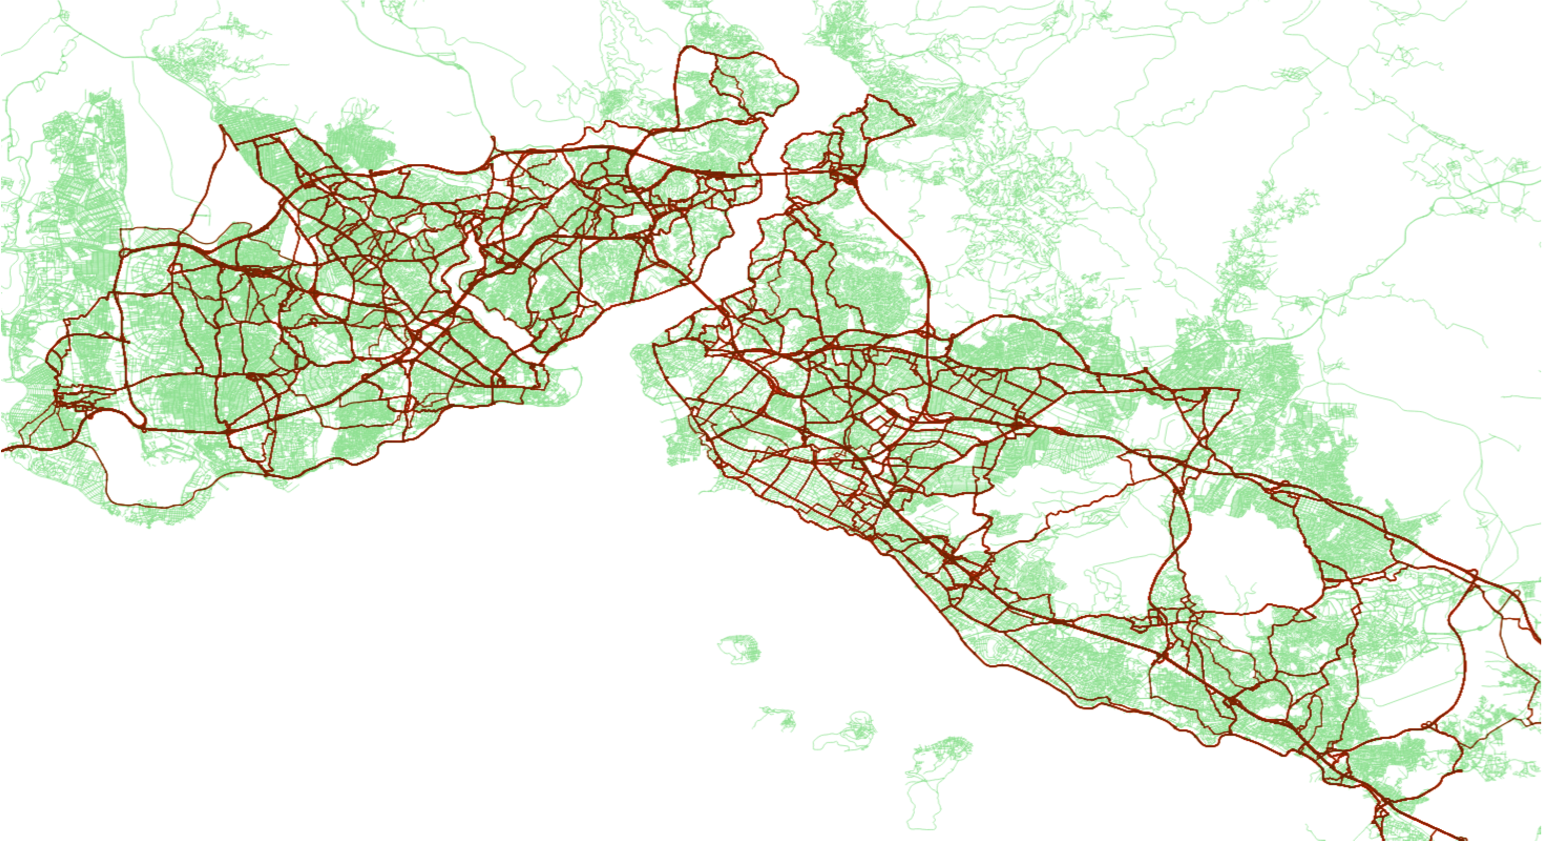
\includegraphics[width=0.45\textwidth]{istanbul}
  \caption{Istanbul road network with chosen routes highlighted}
  \label{istanbul}
\end{figure}
The result of the route choice model can be seen in figure \ref{istanbul}. The map only shows the road network of Istanbul, but it is quite easy to recognise the topography of the city. The Bosphorus strait is visible in the center with the two bridges connecting Europe and Asia. The white spots in the map are mountainous areas, with only a few roads. The overlay with darker color is the routes chosen by the model to serve the origin destination demand matrix. The demand is simulated, by choosing 44 points in Istanbul as origins. The points were chosen at central locations in different parts of the city, where the traffic could easily be dispersed without creating congestion at the origin. The points represents the traffic demand from an area around the chosen point. Each origin creates traffic demand to all other origins,with a constant demand, to create an origin destination matrix with 1892 non zero entries.

The runtime of the algorithm is visualised in figure \ref{runtime}. The figure shows the runtime for one iteration as a function of the number of iterations.
 \begin{figure}[h]
	\centering
  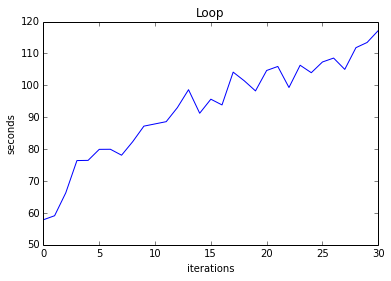
\includegraphics[width=0.45\textwidth]{runtime}
  \caption{Runtime versus iterations}
  \label{runtime}
\end{figure}

The runtime of an iteration increases linearly as the number of iterations increases.

In figure \ref{convergence} the convergence of the algorithm is shown. The error is a measure of the differences in travel times for the different routes for each origin destination pair.
 \begin{figure}[h]
	\centering
  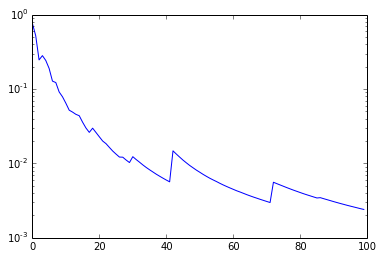
\includegraphics[width=0.45\textwidth]{convergence}
  \caption{Convergence of the model for  the Istanbul case}
  \label{convergence}
\end{figure}

The figure shows how the error decreases fast in the initial steps of the algorithm. The error further decreases more slowly as the algorithm continues. The sudden increases in the error is when a new route is found, with a lower travel time. The route is added to the error calculation without any traffic making the traffic for that origin destination pair unbalanced, and hence contribute with a large error. As the traffic volumes for the different routes is reshuffled, the travel times of the routes move closer to each other, thus reducing the error.
 %                  AAR
%                 HER
 %           Congestion results    
 %                 IST
 %                 AAR /HER

 \begin{figure}[h]
	\centering
  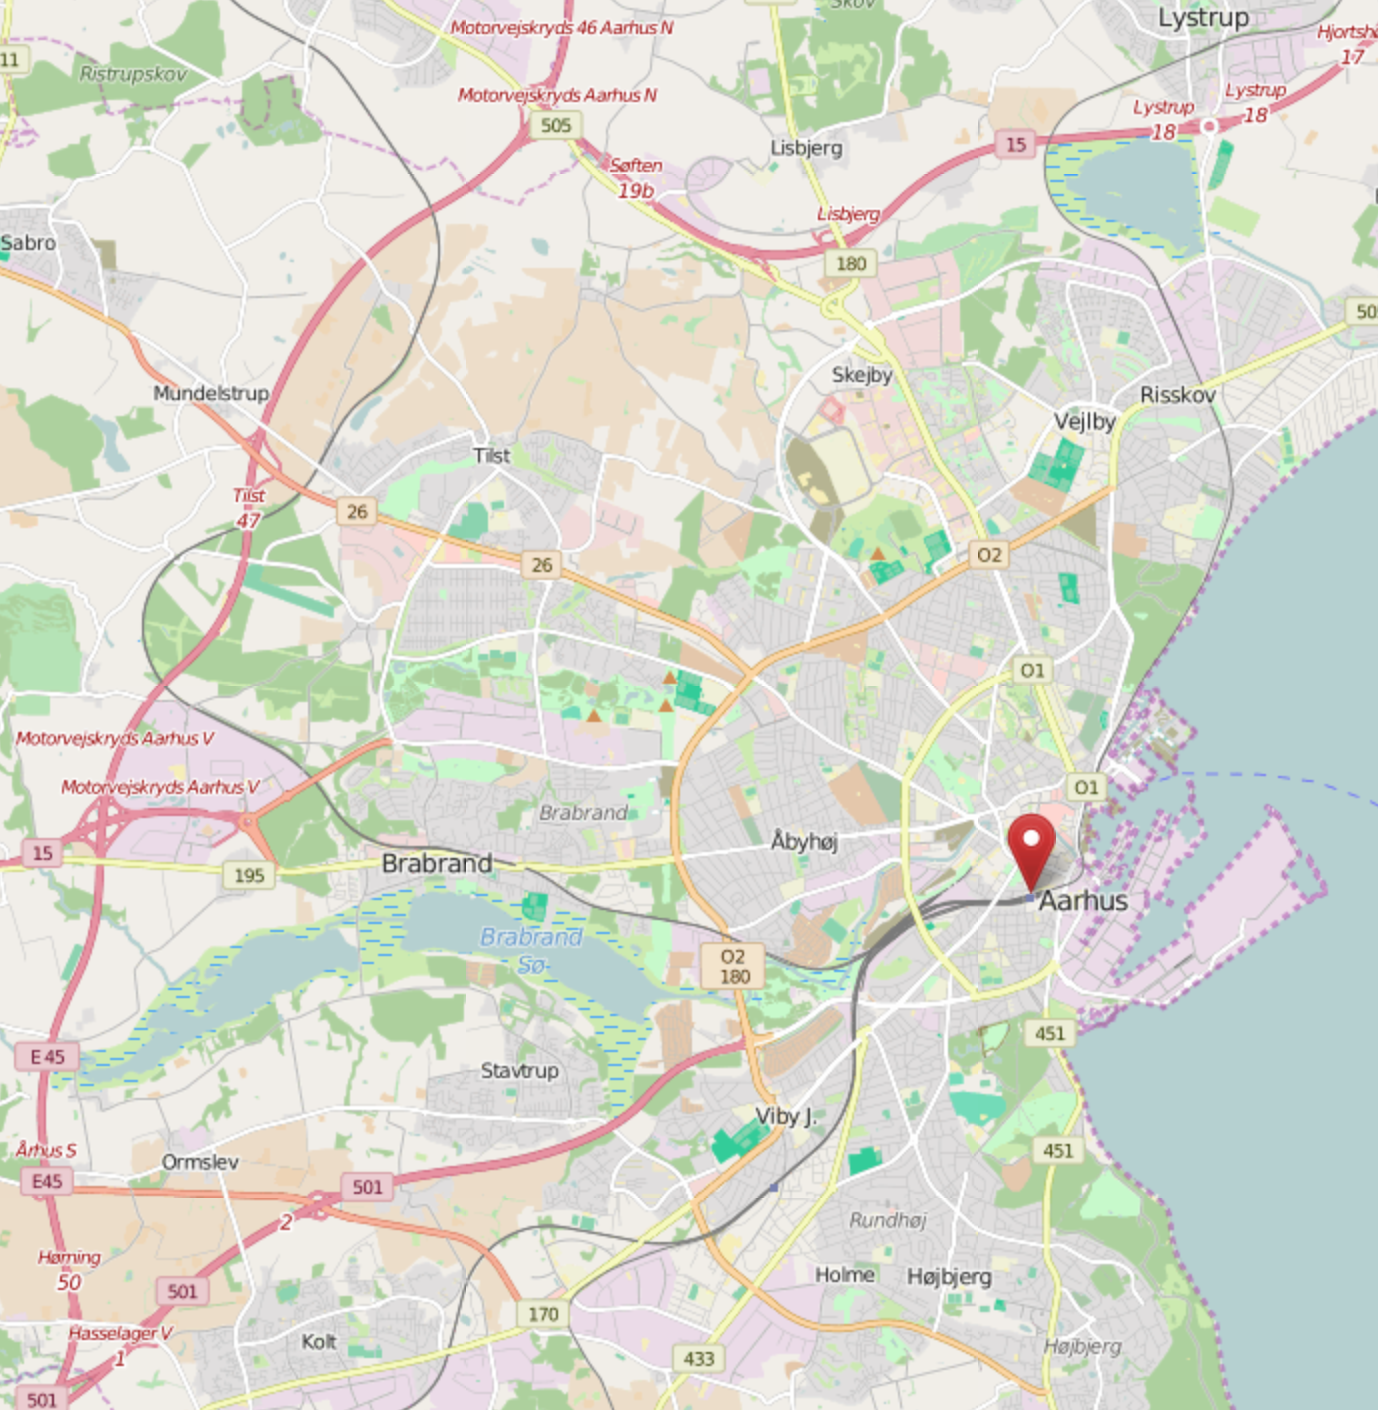
\includegraphics[width=0.45\textwidth]{aarhus}
  \caption{Map of Aarhus}
  \label{aarhus}
\end{figure}
 \begin{figure}[h]
	\centering
  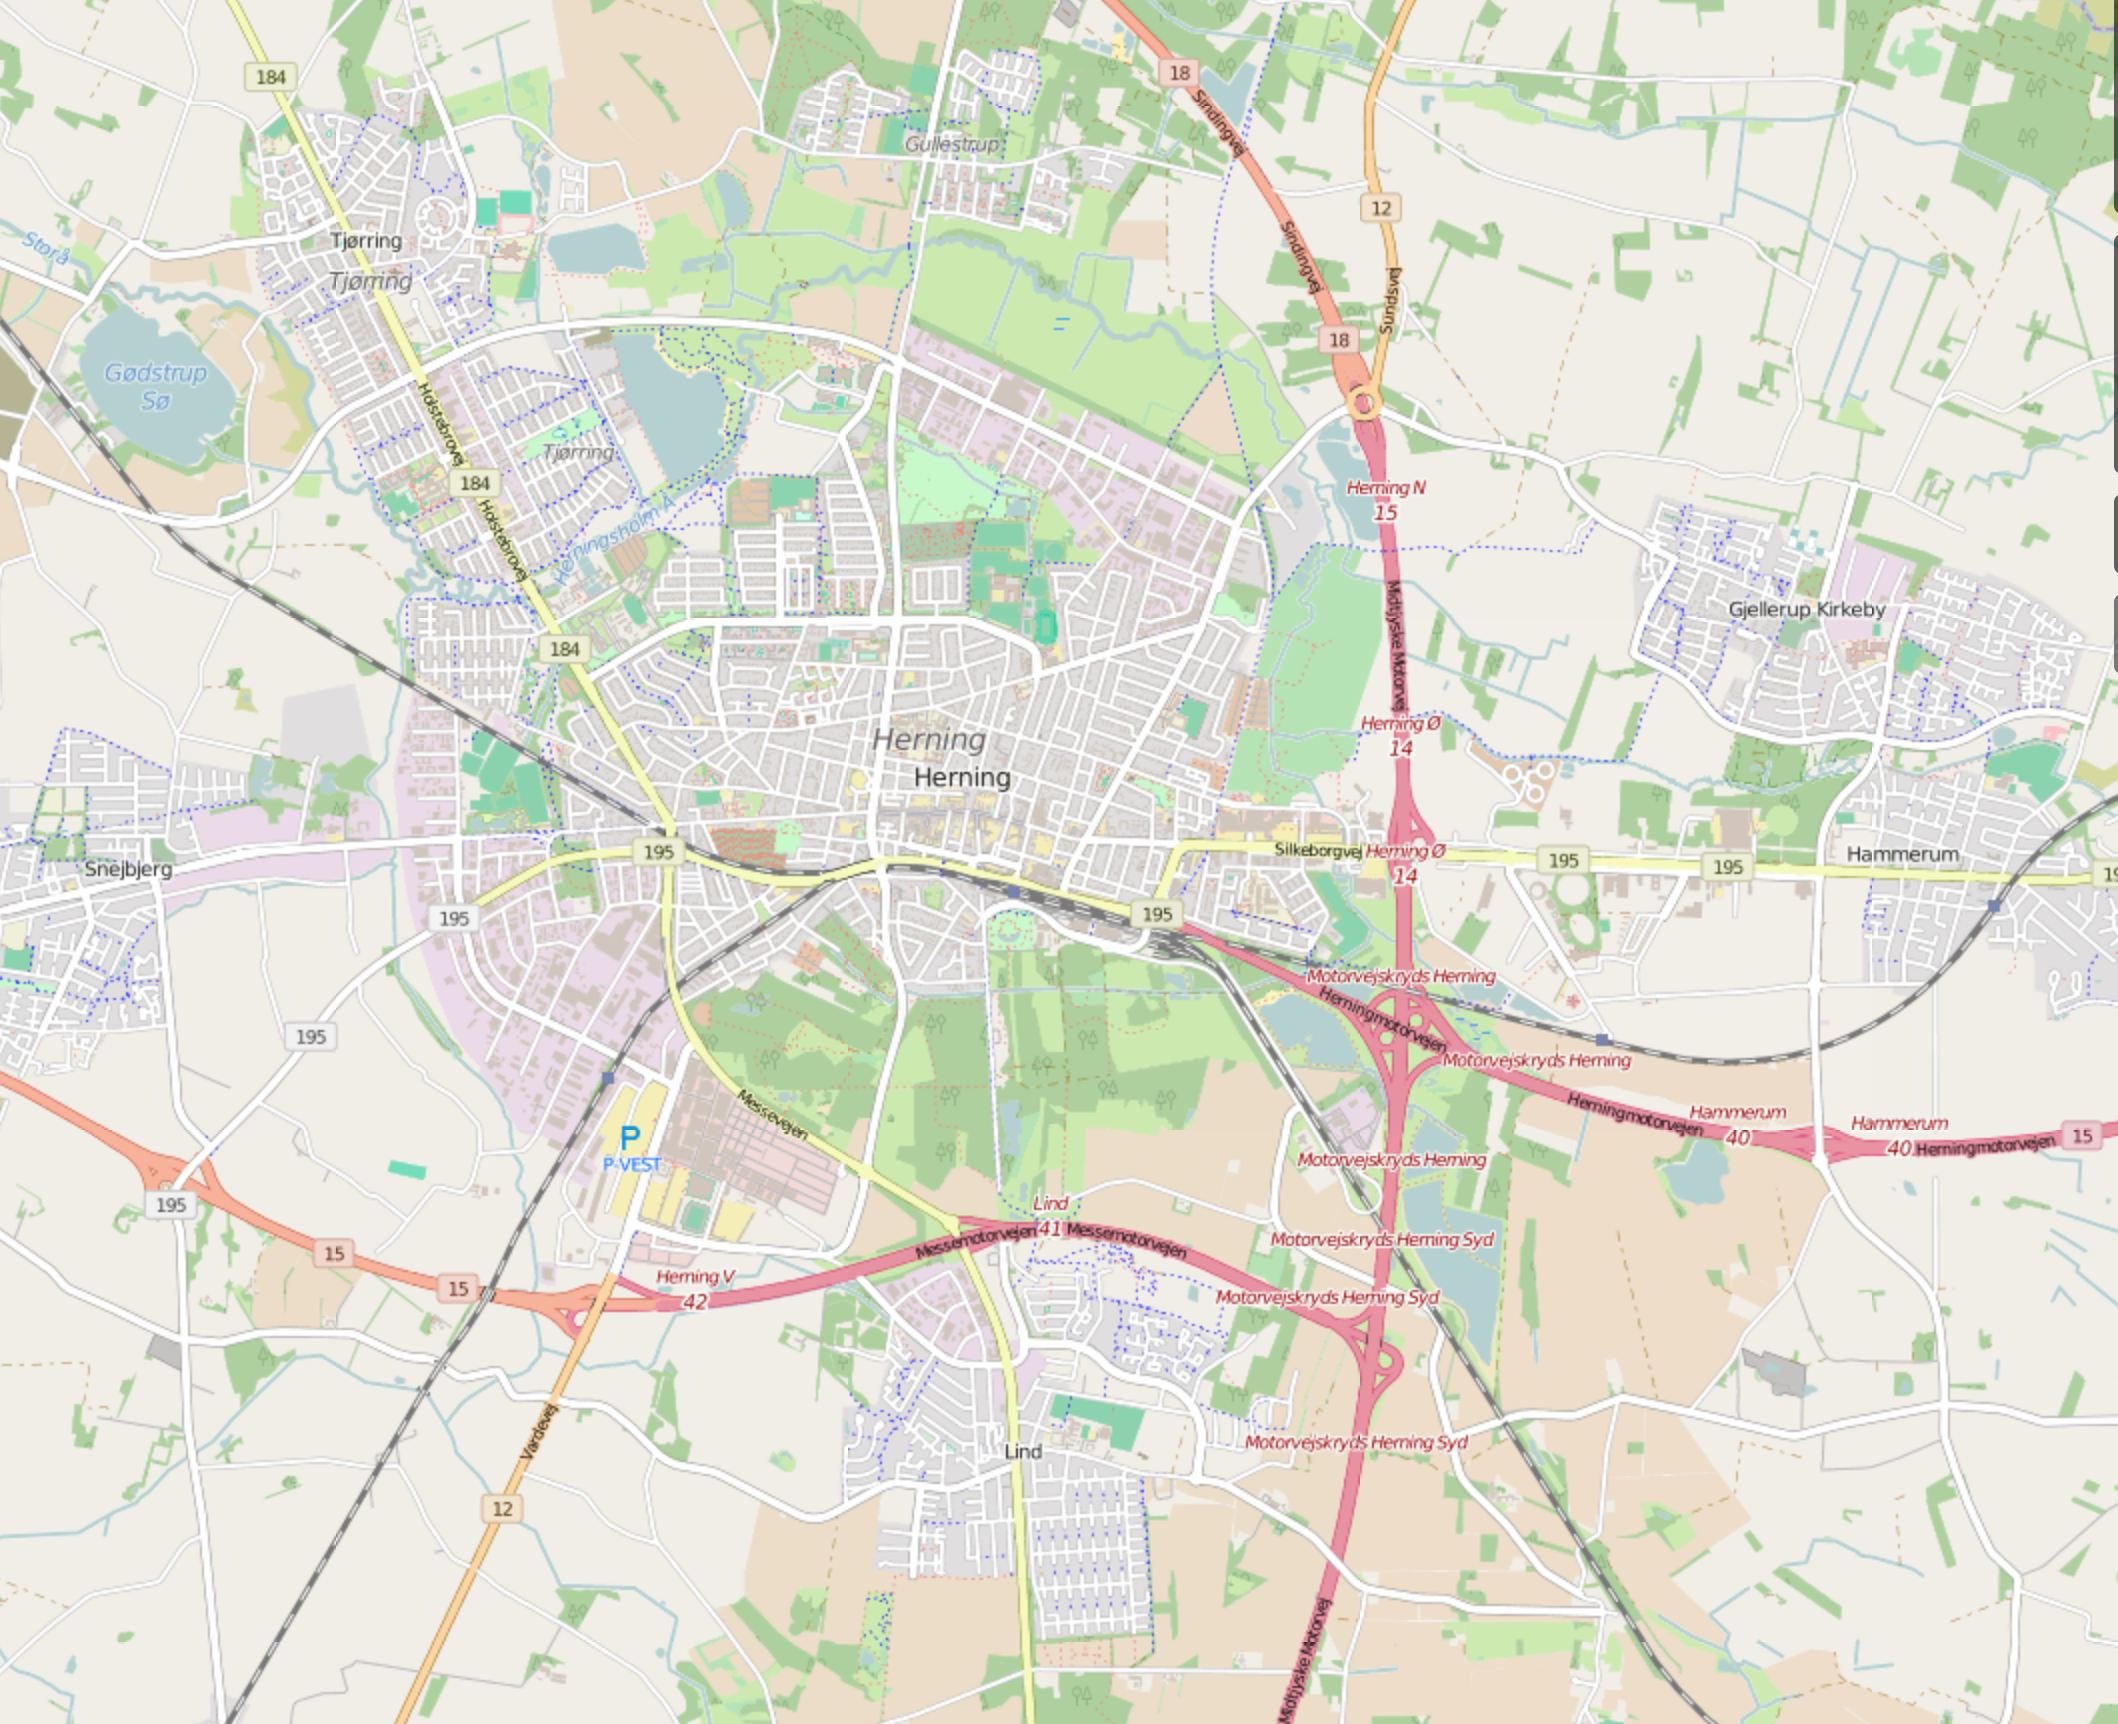
\includegraphics[width=0.45\textwidth]{herning}
  \caption{Map of Herning}
  \label{herning}
\end{figure}

 \section{Further work}
 %       Further work
 To further improve the congestion model, we plan to expand the model to more kinds of traffic, by integration commercial transport of goods, and public transport into the traffic mix. 
 To improve the creation of origin-destination matrix, we want to improve the stochastic model for generating the traffic demand, by adding heuristics based on knowledge gained from local observers, transit data and crowd sensed data.
 Including turn delays and intersection modelling \cite{nielsen1998turn} would further increase the accuracy of the model.
 
 \section{Conclusion}
 In this paper we have presented the efficient database implementation of a congestion model based on the Restricted Stochastic User Equilibrium algorithm. We also presented a method to create demand data for the congestion model, guided by crowd sensed travel data.
 %       Conclusion
 
 % figures :
 %      Visualise results from IST
 %         QGIS ? (better colors)
 %         Show congestion points
 %
 %      
\section*{Acknowledgment}
I large part of this work was done at the Sabanci University, Istanbul, generously supported by professor B�lent �atay.
This work has been supported by The Danish Council for Strategic Research as part of the EcoSense project (11-115331).
%\newpage
%\pagenumbering{gobble}	
\bibliographystyle{abbrv}
\bibliography{casper16}
\end{document}  


